\documentclass[aspectratio=169,11pt,svgnames,draft]{beamer}

\usepackage[english]{babel}
\usepackage{graphicx}
\usepackage{enumitem}
\usepackage{amsmath}
\usepackage{mathtools}
\usepackage{float}
\usepackage{tikz}
\usetikzlibrary{patterns}
\usepackage{tkz-euclide}
\tikzset{point style/.style = {%
  draw = black,
  inner sep = 0pt,
  shape = circle,
  minimum size = 5pt,
  fill = black
 }
}
\usepackage{enumitem}

\usepackage{caption}
\usepackage{subcaption}

% Flowchart stuff

\usepackage{pgfopts}
\usepackage{xcolor}
\usepackage{tcolorbox}

\usetheme[
 titlestyle=style2,
 titleformat=smallcaps,
 sectionstyle=plain,
 slidestyle=cyber,
 headingcolor=theme,
 block=transparent
]{trigon}

\title{Polygons}
\date{\today}
\author{Adam Klepáč}
\institute[GEVO]{Gymnázium Evolution Jižní Město}
\biglogo[width=.2\textwidth]{logo}
\smalllogo[width=.1\textwidth]{logo}
\titlegraphic{
\includegraphics[height=\paperheight]{title.jpg}}

\def\subsectionname{}

% enumerate global settings
\setlist[enumerate,1]{label=\arabic*.}
\setlist[enumerate,2]{label=\alph*)}

% custom colors %
\definecolor{PolygonYellow}{HTML}{f6e01a}
\definecolor{PolygonCyan}{HTML}{11cdef}
\definecolor{PolygonOrange}{HTML}{b25c10}
\definecolor{PolygonBlue}{HTML}{0a2a66}
\colorlet{tPrim}{PolygonBlue}
\colorlet{tTheme}{PolygonYellow}
\colorlet{tSec}{PolygonCyan}
\colorlet{tAccent}{PolygonCyan}

\tcbset{
 boxsep=7pt,
 fonttitle=\sc,
 colframe=tGreyBg,
 colframe=tPrim,
 boxrule=1pt
}

\begin{document}
\titleframe

\begin{frame}
 \frametitle{Contents}
 \tableofcontents
\end{frame}

% \section{General Polygons}
% \label{sec:general-polygons}
%
% \begin{frame}
%  \frametitle{General Polygons -- Def~\hspace{-.4ex}inition}
%  \begin{tcolorbox}[title=Polygon]
%   A \alert{polygon} is a closed 2D shape made of only segments.
%  \end{tcolorbox}
%  \begin{itemize}
%   \item<2-> The endpoints of those segments are called \alert{vertices}.
%   \item<3-> The segments themselves are called \alert{edges}.
%  \end{itemize}
% \end{frame}
%
% \begin{frame}
%  \frametitle{General Polygons -- Examples}
%  \begin{figure}[H]
%   \centering
%   \begin{subfigure}[b]{.23\textwidth}
%    \centering
%    \begin{tikzpicture}
%     \tkzDefPoint(0:1){A}
%     \tkzDefPoint(110:2){B}
%     \tkzDefPoint(180:1){C}
%
%     \tkzDrawPoints(A,B,C);
%     \tkzDrawSegments(A,B B,C C,A);
%    \end{tikzpicture}
%    \caption*{Triangle}
%   \end{subfigure}
%   \begin{subfigure}[b]{.23\textwidth}
%    \centering
%    \begin{tikzpicture}
%     \tkzDefPoint(0:1){A}
%     \tkzDefPoint(60:1.5){B}
%     \tkzDefPoint(130:2.5){C}
%     \tkzDefPoint(180:1){D}
%
%     \tkzDrawPoints(A,B,C, D);
%     \tkzDrawSegments(A,B B,C C,D D,A);
%    \end{tikzpicture}
%    \caption*{Quadrilateral}
%   \end{subfigure}
%   \begin{subfigure}[b]{.23\textwidth}
%    \centering
%    \begin{tikzpicture}
%     \tkzDefPoint(0:1){A}
%     \tkzDefPoint(50:2){B}
%     \tkzDefPoint(90:2){C}
%     \tkzDefPoint(120:2){D}
%     \tkzDefPoint(180:1){E}
%
%     \tkzDrawPoints(A,B,C,D,E);
%     \tkzDrawSegments(A,B B,C C,D D,E E,A);
%    \end{tikzpicture}
%    \caption*{Pentagon}
%   \end{subfigure}
%   \begin{subfigure}[b]{.27\textwidth}
%    \centering
%    \begin{tikzpicture}
%     \tkzDefPoint(0:1){A}
%     \tkzDefPoint(13:2){B}
%     \tkzDefPoint(30:2.5){C}
%     \tkzDefPoint(50:2){D}
%     \tkzDefPoint(70:1){E}
%     \tkzDefPoint(86:2){F}
%     \tkzDefPoint(97:1.5){G}
%     \tkzDefPoint(109:2){H}
%     \tkzDefPoint(121:2){I}
%     \tkzDefPoint(140:1.5){J}
%     \tkzDefPoint(160:1){K}
%     \tkzDefPoint(180:1){L}
%
%     \tkzDrawPoints(A,B,C,D,E,F,G,H,I,J,K,L);
%     \tkzDrawSegments(A,B B,C C,D D,E E,F F,G G,H H,I I,J J,K K,L L,A);
%    \end{tikzpicture}
%    \caption*{Dodecagon}
%   \end{subfigure}
%  \end{figure}
%  \begin{itemize}
%   \item <2-> A polygon with $n \in \mathbb{N}$ sides is called an $n$-gon.
%   \item <3-> For example a polygon with 123456 sides is called a $123456$-gon or
%    decadismyriatrischilliatetrahectapentacontakaihexagon.
%  \end{itemize} 
% \end{frame}
%
% \begin{frame}
%  \frametitle{General Polygons -- Counterexamples}
%  \begin{figure}[H]
%   \centering
%   \begin{subfigure}[b]{.33\textwidth}
%    \centering
%    \begin{tikzpicture}
%     \tkzDefPoint(0:1){A}
%     \tkzDefPoint(90:1){B}
%     \tkzDefPoint(150:1){C}
%
%     \tkzDrawPoints(A,B,C);
%     \tkzDrawSegments(A,B B,C);
%    \end{tikzpicture}
%    \caption*{Not closed}
%   \end{subfigure}
%   \begin{subfigure}[b]{.33\textwidth}
%    \centering
%    \begin{tikzpicture}[scale=2]
%     \tkzDefPoint(0,0){A1}
%     \tkzDefPoint(0,1){B1}
%     \tkzDefPoint(1,1){C1}
%     \tkzDefPoint(1,0){D1}
%
%     \tkzDefPoint(0.5,0.3){A2}
%     \tkzDefPoint(0.5,1.3){B2}
%     \tkzDefPoint(1.5,1.3){C2}
%     \tkzDefPoint(1.5,0.3){D2}
%     \tkzDrawPoints(A1,B1,C1,D1,A2,B2,C2,D2)
%
%     \tkzDrawSegments(A1,B1 B1,C1 C1,D1 D1,A1 B2,C2 C2,D2 B1,B2 C1,C2 D1,D2)
%     \tkzDrawSegments[dashed](A2,B2 D2,A2 A1,A2)
%    \end{tikzpicture}
%    \caption*{3D}
%   \end{subfigure}
%   \begin{subfigure}[b]{.33\textwidth}
%    \centering
%    \begin{tikzpicture}
%     \tkzDefPoint(0:1){A}
%     \tkzDefPoint(180:1){B}
%     \tkzDefPoint(90:1){P}
%
%     \tkzDrawPoints(A,B)
%     \tkzDrawArc(P,A)(B)
%     \tkzDrawSegment(A,B)
%    \end{tikzpicture}
%    \caption*{Not straight}
%   \end{subfigure}
%  \end{figure}
% \end{frame}
%
% \begin{frame}
%  \frametitle{General Polygons -- Convexity}
%  \begin{tcolorbox}[title=Convex Polygon]
%   A polygon is called \alert{convex} if it has no internal angle greater than
%   180$^{\circ}$.
%  \end{tcolorbox}
%  \pause
%  \begin{figure}[H]
%   \centering
%   \begin{subfigure}[b]{.45\textwidth}
%    \centering
%    \begin{tikzpicture}
%     \tkzDefPoint(0:1){A}
%     \tkzDefPoint(50:2){B}
%     \tkzDefPoint(90:2){C}
%     \tkzDefPoint(120:2){D}
%     \tkzDefPoint(180:1){E}
%
%     \tkzDrawPoints[color=ForestGreen](A,B,C,D,E);
%     \tkzDrawSegments[color=ForestGreen](A,B B,C C,D D,E E,A);
%    \end{tikzpicture}
%    \caption*{\textcolor{ForestGreen}{Convex}}
%   \end{subfigure}
%   \begin{subfigure}[b]{.45\textwidth}
%    \centering
%    \begin{tikzpicture}
%     \tkzDefPoint(0,0){A}
%     \tkzDefPoint(2,0){B}
%     \tkzDefPoint(2,2){C}
%     \tkzDefPoint(1,1){D}
%     \tkzDefPoint(0,2){E}
%
%     \tkzDrawPoints[color=Red](A,B,C,D,E)
%     \tkzDrawSegments[color=Red](A,B B,C C,D D,E E,A)
%
%     \tkzMarkAngle[color=Red,size=0.65](E,D,C)
%     \tkzLabelAngle[color=Red,pos=0.25](E,D,C){\footnotesize $>\!\!180^{ \circ}$}
%    \end{tikzpicture}
%    \caption*{\textcolor{Red}{NOT convex}}
%   \end{subfigure}
%  \end{figure}
% \end{frame}
%
% \section{Convex Polygons}
% \label{sec:convex-polygons}
%
% \begin{frame}
%  \frametitle{Convex Polygons -- Special Types}
%  \begin{figure}[H]
%   \centering
%   \begin{subfigure}[b]{.33\textwidth}
%    \begin{tikzpicture}[scale=2]
%     \tkzDefPoint(0,0){A}
%     \tkzDefPoint(0.3,1){B}
%     \tkzDefPoint(1,1){C}
%     \tkzDefPoint(2,0){D}
%
%     \tkzDrawPolygon(A,B,C,D)
%     \tkzDrawSegments[ultra thick,PolygonCyan](B,C A,D)
%     \tkzDrawPoints(A,B,C,D)
%    \end{tikzpicture}
%    \caption*{\alert{Trapezoid/Trapezium}\\
%     A convex quadrilateral with at least two
%    parallel sides.}
%   \end{subfigure}
%   \pause
%   \begin{subfigure}[b]{.33\textwidth}
%    \begin{tikzpicture}[scale=2]
%     \tkzDefPoint(0,0){A}
%     \tkzDefPoint(0.5,0.75){B}
%     \tkzDefPoint(2,0.75){C}
%     \tkzDefPoint(1.5,0){D}
%
%     \tkzDrawSegments[ultra thick,PolygonCyan](B,C A,D)
%     \tkzDrawSegments[ultra thick,PolygonOrange](A,B C,D)
%     \tkzDrawPoints(A,B,C,D)
%    \end{tikzpicture}
%    \caption*{\alert{Parallelogram}\\
%     A convex quadrilateral with two pairs of
%    parallel sides.}
%   \end{subfigure}
%   \pause
%   \begin{subfigure}[b]{.33\textwidth}
%    \begin{tikzpicture}[scale=2]
%     \clip (-0.04,-0.04) rectangle (1.44,0.79);
%     \tkzDefPoint(0,0){A}
%     \tkzDefPoint(0.5,0.75){B}
%     \tkzDefPoint(1.4,0.75){C}
%     \tkzDefPoint(0.9,0){D}
%
%     \tkzDrawPolygon[ultra thick,PolygonBlue!75](A,B,C,D)
%     \tkzDrawPoints(A,B,C,D)
%     \tkzDrawSegments[thick](A,C B,D)
%     \tkzInterLL(A,C)(B,D) \tkzGetPoint{O}
%     \tkzMarkAngle[size=0.2](A,O,D)
%     \tkzLabelAngle[pos=0.1](A,O,D){$ \cdot $}
%    \end{tikzpicture}
%    \caption*{\alert{Rhombus}\\
%    An \textbf{equilateral} (all sides of the same length) parallelogram.}
%   \end{subfigure}
%  \end{figure}
% \end{frame}
%
% \begin{frame}
%  \frametitle{Convex Polygons -- Diagonals}
%  \begin{tcolorbox}[title=Diagonal in A Convex Polygon]
%   A \alert{diagonal} of a \textbf{convex} polygon is a segment connecting two of
%   its non-adjacent vertices.
%  \end{tcolorbox}
%  \begin{minipage}[c][4cm][c]{0.48\textwidth}
%   \begin{figure}[H]
%    \centering
%    \begin{tikzpicture}
%     \tkzDefPoint(0,0){A}
%     \tkzDefPoint(-1,0.5){B}
%     \tkzDefPoint(0.3,2){C}
%     \tkzDefPoint(2,1){D}
%     \tkzDefPoint(2,0.5){E}
%     \tkzDefPoint(1.5,0){F}
%     \tkzDrawPolygon(A,B,C,D,E,F)
%     \tkzDrawSegment[color=PolygonCyan,ultra thick](A,D)
%     \tkzDrawPoints(A,B,C,D,E,F)
%    \end{tikzpicture}
%    \caption*{\textcolor{PolygonCyan}{Diagonal} in a convex hexagon.}
%   \end{figure}
%  \end{minipage}
%  \pause
%  \begin{minipage}[c][4cm][c]{.48\textwidth}
%   \vspace*{\fill}
%   \textcolor{PolygonOrange}{\textbf{Voluntary HW}}: How many different diagonals
%   does a convex $n$-gon have?
%   \vspace*{\fill}
%  \end{minipage}
% \end{frame}
%
% \begin{frame}
%  \frametitle{Convex Polygons -- Triangulations}
%  \begin{tcolorbox}[title=Triangulation of A Convex Polygon]
%   A \alert{triangulation} of a \textbf{convex} polygon is its division into
%   triangles by non-intersecting diagonals.
%  \end{tcolorbox}
%  \pause
%  \begin{figure}[H]
%   \centering
%   \begin{subfigure}[b]{.2\textwidth}
%    \centering
%    \begin{tikzpicture}[scale=0.875]
%     \tkzDefPoint(-45:1){A}
%     \tkzDefPoint(-135:1){B}
%     \tkzDefPoint(135:1){C}
%     \tkzDefPoint(45:1){D}
%
%     \tkzDrawPolygon(A,B,C,D)
%     \tkzDrawSegment[ultra thick,PolygonCyan](A,C)
%     \tkzDrawPoints(A,B,C,D)
%    \end{tikzpicture}
%   \end{subfigure}
%   \begin{subfigure}[b]{.2\textwidth}
%    \centering
%    \begin{tikzpicture}[scale=0.7]
%     \tkzDefPoint(0:1){A}
%     \tkzDefPoint(60:1){B}
%     \tkzDefPoint(120:1){C}
%     \tkzDefPoint(180:1){D}
%     \tkzDefPoint(240:1){E}
%     \tkzDefPoint(300:1){F}
%
%     \tkzDrawPolygon(A,B,C,D,E,F)
%     \tkzDrawSegments[ultra thick,color=PolygonCyan](A,C D,F A,D)
%     \tkzDrawPoints(A,B,C,D,E,F)
%    \end{tikzpicture}
%   \end{subfigure}
%   \begin{subfigure}[b]{.2\textwidth}
%    \centering
%    \begin{tikzpicture}[scale=0.7]
%     \tkzDefPoint(0:1){A}
%     \tkzDefPoint(60:1){B}
%     \tkzDefPoint(120:1){C}
%     \tkzDefPoint(180:1){D}
%     \tkzDefPoint(240:1){E}
%     \tkzDefPoint(300:1){F}
%
%     \tkzDrawPolygon(A,B,C,D,E,F)
%     \tkzDrawSegments[ultra thick,color=PolygonCyan](B,D D,F B,F)
%     \tkzDrawPoints(A,B,C,D,E,F)
%    \end{tikzpicture}
%   \end{subfigure}
%   \caption*{Examples of \textcolor{PolygonCyan}{triangulations}.}
%  \end{figure}
%  \vspace*{-1em}
%  \pause
%  \textcolor{PolygonOrange}{\textbf{Voluntary HW}}: How many different
%  triangulations of an $n$-gon are there?
% \end{frame}
%
% \begin{frame}
%  \frametitle{Convex Polygons -- Triangulations}
%  \begin{tcolorbox}[title=Triangulation of A Convex Polygon]
%   A \alert{triangulation} of a \textbf{convex} polygon is its division into
%   triangles by non-intersecting diagonals.
%  \end{tcolorbox}
%  \begin{figure}[H]
%   \centering
%   \begin{subfigure}[b]{.2\textwidth}
%    \centering
%    \begin{tikzpicture}[scale=0.875]
%     \tkzDefPoint(-45:1){A}
%     \tkzDefPoint(-135:1){B}
%     \tkzDefPoint(135:1){C}
%     \tkzDefPoint(45:1){D}
%
%     \tkzDrawPolygon(A,B,C,D)
%     \tkzDrawSegment[ultra thick,PolygonCyan](A,C)
%     \tkzDrawPoints(A,B,C,D)
%    \end{tikzpicture}
%   \end{subfigure}
%   \begin{subfigure}[b]{.2\textwidth}
%    \centering
%    \begin{tikzpicture}[scale=0.7]
%     \tkzDefPoint(0:1){A}
%     \tkzDefPoint(60:1){B}
%     \tkzDefPoint(120:1){C}
%     \tkzDefPoint(180:1){D}
%     \tkzDefPoint(240:1){E}
%     \tkzDefPoint(300:1){F}
%
%     \tkzDrawPolygon(A,B,C,D,E,F)
%     \tkzDrawSegments[ultra thick,color=PolygonCyan](A,C D,F A,D)
%     \tkzDrawPoints(A,B,C,D,E,F)
%    \end{tikzpicture}
%   \end{subfigure}
%   \begin{subfigure}[b]{.2\textwidth}
%    \centering
%    \begin{tikzpicture}[scale=0.7]
%     \tkzDefPoint(0:1){A}
%     \tkzDefPoint(60:1){B}
%     \tkzDefPoint(120:1){C}
%     \tkzDefPoint(180:1){D}
%     \tkzDefPoint(240:1){E}
%     \tkzDefPoint(300:1){F}
%
%     \tkzDrawPolygon(A,B,C,D,E,F)
%     \tkzDrawSegments[ultra thick,color=PolygonCyan](B,D D,F B,F)
%     \tkzDrawPoints(A,B,C,D,E,F)
%    \end{tikzpicture}
%   \end{subfigure}
%   \caption*{Examples of \textcolor{PolygonCyan}{triangulations}.}
%  \end{figure}
%  \vspace*{-1em}
%  \textcolor{PolygonOrange}{\textbf{Voluntary HW}}: Find a \textbf{non-convex}
%  polygon which \textbf{cannot} be triangulated.
% \end{frame}
%
% \begin{frame}
%  \frametitle{Convex Polygons -- Internal Angles}
%  \begin{figure}[H]
%   \begin{tikzpicture}
%    \tkzDefPoint(-54:1){A};
%    \tkzDefPoint(18:1){B};
%    \tkzDefPoint(90:1){C};
%    \tkzDefPoint(162:1){D};
%    \tkzDefPoint(234:1){E};
%
%    \tkzDrawPolygon(A,B,C,D,E);
%    \tkzDrawPoints(A,B,C,D,E);
%    \tkzMarkAngle[size=0.4,Red,thick](B,A,E)
%    \tkzMarkAngle[size=0.4,Red,thick](A,E,D)
%    \tkzMarkAngle[size=0.4,Red,thick](E,D,C)
%    \tkzMarkAngle[size=0.4,Red,thick](D,C,B)
%    \tkzMarkAngle[size=0.4,Red,thick](C,B,A)
%   \end{tikzpicture}
%   \caption*{\textcolor{Red}{\textbf{Internal angles}} of a pentagon.}
%  \end{figure}
%  \textbf{Question:} What is the sum of internal angles of a convex $n$-gon?
%  \begin{itemize}[label=\textbullet]
%   \item<2-> For a triangle, it's 180$^{ \circ }$.
%   \item<3-> For a square, it's 360$^{\circ}$.
%   \item<4-> For a pentagon, it's 540$^{ \circ }$.
%  \end{itemize}
% \end{frame}
%
% \begin{frame}
%  \frametitle{Convex Polygons -- Internal Angles}
%  \begin{itemize}
%   \item We can count internal angles using triangulations.
%   \pause
%   \item Into how many triangles is a convex $n$-gon divided?
%   \pause
%   \item Each triangle shares two vertices with an adjacent one.
%   \pause
%   \item We choose the first triangle -- it covers 3 vertices.
%   \pause
%   \item After that, each triangle covers only one more vertex.
%   \pause
%   \item This means, that an $n$-gon is divided into $n-2$ triangles.
%  \end{itemize}
%  \begin{figure}[H]
%   \pause
%   \begin{subfigure}[b]{.24\textwidth}
%    \centering
%    \begin{tikzpicture}
%     \tkzDefPoint(0:1){A}
%     \tkzDefPoint(60:1){B}
%     \tkzDefPoint(120:1){C}
%     \tkzDefPoint(180:1){D}
%     \tkzDefPoint(240:1){E}
%     \tkzDefPoint(300:1){F}
%
%     \tkzDrawPolygon(A,B,C,D,E,F)
%     \tkzDrawSegment[ultra thick,color=PolygonCyan](B,D)
%     \tkzDrawPolygon[fill=PolygonCyan!30](B,C,D)
%     \tkzDrawPoints(A,E,F)
%     \tkzDrawPoints[color=PolygonCyan](B,C,D)
%    \end{tikzpicture}
%   \end{subfigure}
%   \begin{subfigure}[b]{.24\textwidth}
%    \centering
%    \begin{tikzpicture}
%     \tkzDefPoint(0:1){A}
%     \tkzDefPoint(60:1){B}
%     \tkzDefPoint(120:1){C}
%     \tkzDefPoint(180:1){D}
%     \tkzDefPoint(240:1){E}
%     \tkzDefPoint(300:1){F}
%
%     \tkzDrawPolygon(A,B,C,D,E,F)
%     \tkzDrawPolygon[fill=PolygonCyan!30](B,C,D)
%     \tkzDrawPolygon[fill=PolygonCyan!30](A,B,D)
%     \tkzDrawSegment[ultra thick,color=PolygonCyan](B,D)
%     \tkzDrawSegment[ultra thick,color=PolygonCyan](A,D)
%     \tkzDrawPoints(E,F)
%     \tkzDrawPoints[color=PolygonCyan](A,B,C,D)
%    \end{tikzpicture}
%   \end{subfigure}
%   \begin{subfigure}[b]{.24\textwidth}
%    \centering
%    \begin{tikzpicture}
%     \tkzDefPoint(0:1){A}
%     \tkzDefPoint(60:1){B}
%     \tkzDefPoint(120:1){C}
%     \tkzDefPoint(180:1){D}
%     \tkzDefPoint(240:1){E}
%     \tkzDefPoint(300:1){F}
%
%     \tkzDrawPolygon(A,B,C,D,E,F)
%     \tkzDrawPolygon[fill=PolygonCyan!30](B,C,D)
%     \tkzDrawPolygon[fill=PolygonCyan!30](A,B,D)
%     \tkzDrawPolygon[fill=PolygonCyan!30](A,D,E)
%     \tkzDrawSegment[ultra thick,color=PolygonCyan](B,D)
%     \tkzDrawSegment[ultra thick,color=PolygonCyan](A,D)
%     \tkzDrawSegment[ultra thick,color=PolygonCyan](A,E)
%     \tkzDrawPoints(F)
%     \tkzDrawPoints[color=PolygonCyan](A,B,C,D,E)
%    \end{tikzpicture}
%   \end{subfigure}
%   \begin{subfigure}[b]{.24\textwidth}
%    \centering
%    \begin{tikzpicture}
%     \tkzDefPoint(0:1){A}
%     \tkzDefPoint(60:1){B}
%     \tkzDefPoint(120:1){C}
%     \tkzDefPoint(180:1){D}
%     \tkzDefPoint(240:1){E}
%     \tkzDefPoint(300:1){F}
%
%     \tkzDrawPolygon(A,B,C,D,E,F)
%     \tkzDrawPolygon[fill=PolygonCyan!30](B,C,D)
%     \tkzDrawPolygon[fill=PolygonCyan!30](A,B,D)
%     \tkzDrawPolygon[fill=PolygonCyan!30](A,D,E)
%     \tkzDrawPolygon[fill=PolygonCyan!30](A,E,F)
%     \tkzDrawSegment[ultra thick,color=PolygonCyan](B,D)
%     \tkzDrawSegment[ultra thick,color=PolygonCyan](A,D)
%     \tkzDrawSegment[ultra thick,color=PolygonCyan](A,E)
%     \tkzDrawPoints[color=PolygonCyan](A,B,C,D,E,F)
%    \end{tikzpicture}
%   \end{subfigure}
%   \caption*{Construction of a \textcolor{PolygonCyan}{triangulation} of a
%   hexagon.}
%  \end{figure}
% \end{frame}
%
% \begin{frame}
%  \frametitle{Convex Polygons -- Internal Angles}
%  \begin{itemize}
%   \item A convex $n$-gon is divided into $n-2$ triangles.
%   \pause
%   \item The sum of all internal angles in a triangle is 180$^{ \circ }$.
%  \end{itemize}
%  \pause
%  \begin{tcolorbox}[title=Sum of Internal Angles in a Convex Polygon]
%   The sum of all internal angles of a convex $n$-gon is $(n-2) \cdot 180^{ \circ
%   }$.
%  \end{tcolorbox}
% \end{frame}

\section{Regular Polygons}

\begin{frame}
 \frametitle{Def~\hspace*{-.4ex}inition}
 \begin{tcolorbox}[title=Regular Polygon]
  A \alert{regular polygon} is a convex polygon whose sides all have the same
  length and whose internal angles all have the same size.
 \end{tcolorbox}
 \begin{figure}[H]
  \centering
  \begin{subfigure}[t]{.24\textwidth}
   \centering
   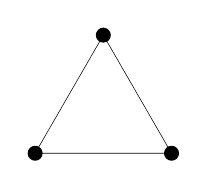
\begin{tikzpicture}
    \tkzDefPoint(-30:1){A}
    \tkzDefPoint(90:1){B}
    \tkzDefPoint(210:1){C}
     
    \tkzDrawPolygon(A,B,C)
    \tkzDrawPoints(A,B,C)
   \end{tikzpicture}
   \caption*{Equilateral triangle (regular trigon)}
  \end{subfigure}
  \begin{subfigure}[t]{.24\textwidth}
   \centering
   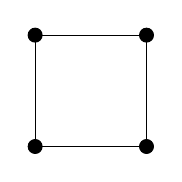
\begin{tikzpicture}
    \tkzDefPoint(-45:1){A}
    \tkzDefPoint(-135:1){B}
    \tkzDefPoint(135:1){C}
    \tkzDefPoint(45:1){D}
     
    \tkzDrawPolygon(A,B,C,D)
    \tkzDrawPoints(A,B,C,D)
   \end{tikzpicture}
   \caption*{Square (regular tetragon)}
  \end{subfigure}
 \end{figure}
\end{frame}

\end{document}
